\documentclass[border=10pt]{standalone}
\usepackage[svgnames]{xcolor}
\usepackage{amsmath}
\usepackage{pgfplots}
\pgfplotsset{compat=newest}
\usepackage[sfdefault]{FiraSans}
\usepackage{FiraMono}
\renewcommand*\familydefault{\sfdefault}
\begin{document}
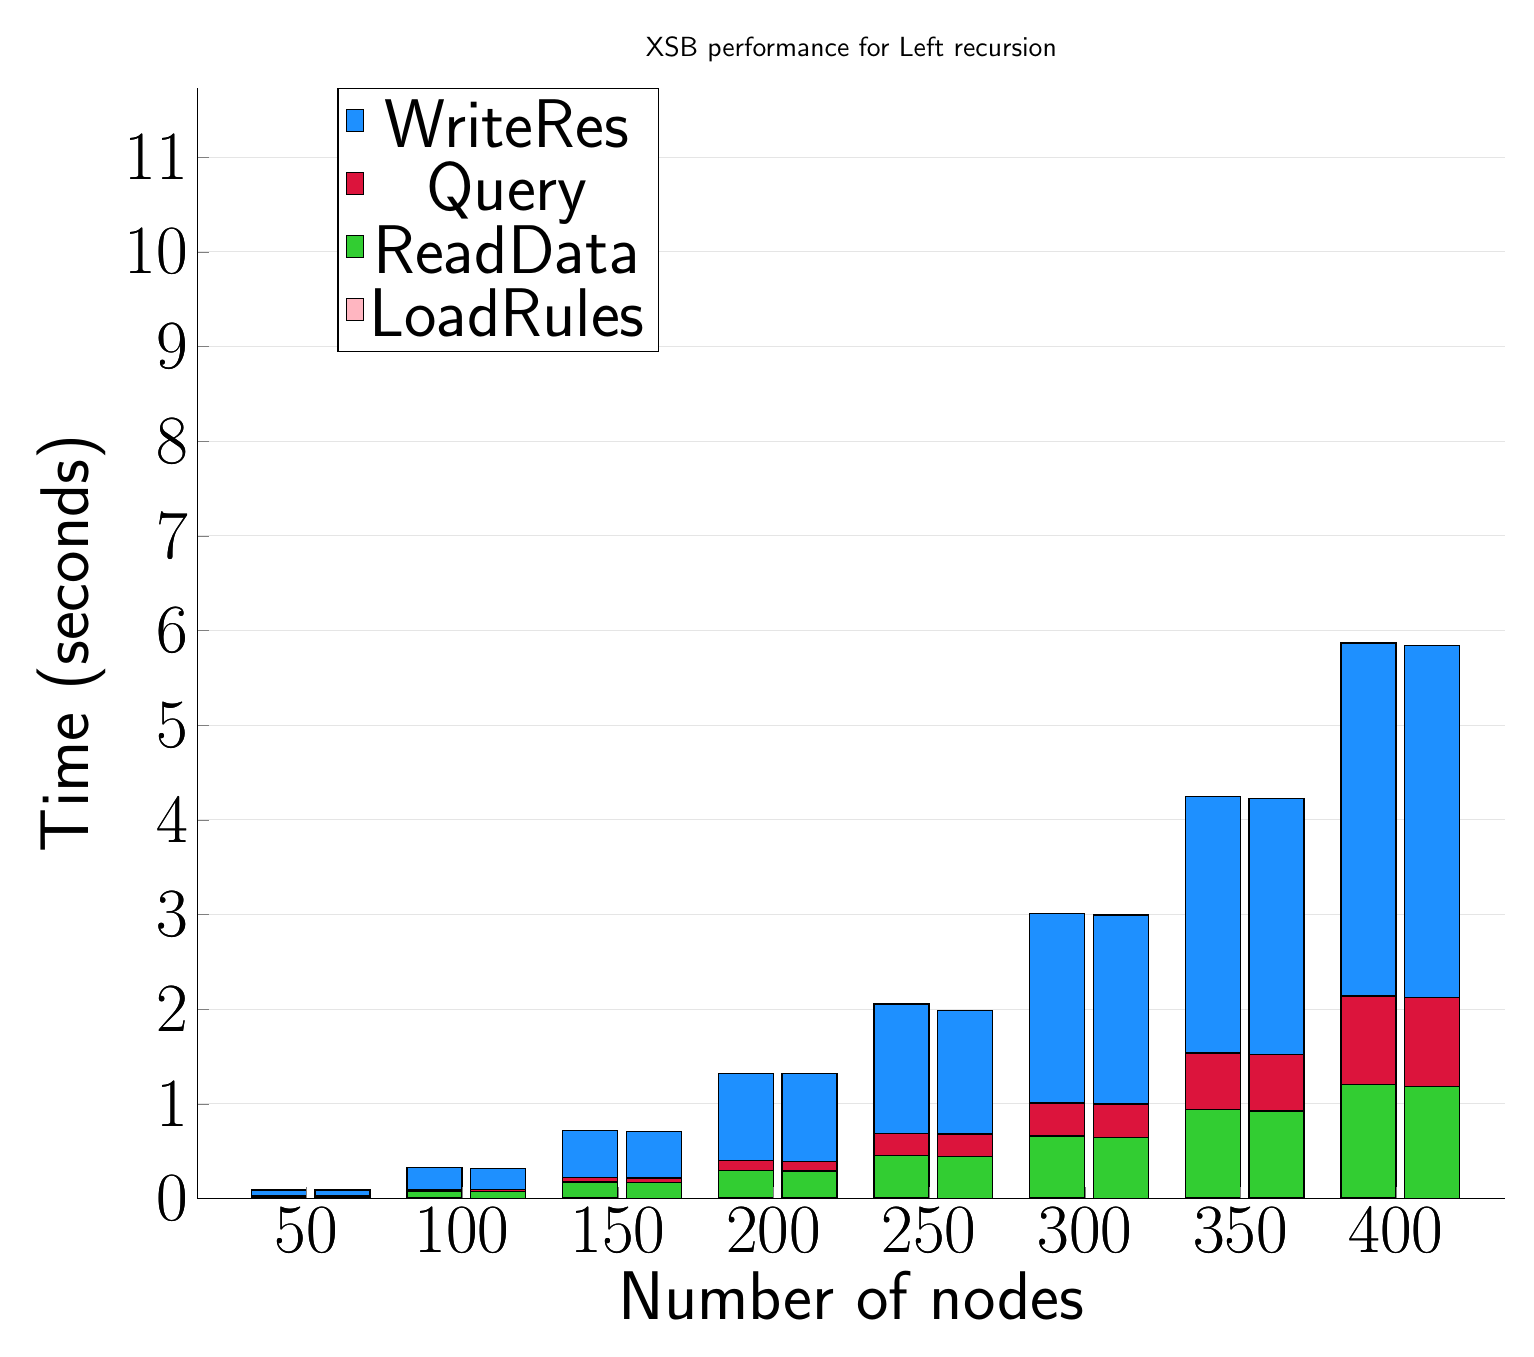
\begin{tikzpicture}
\begin{axis}[
   ybar stacked,
   title={XSB performance for Left recursion},
   bar shift=-10pt,
   width=1.5\textwidth,
   bar width=0.7cm,
   ymajorgrids, tick align=inside,
   major grid style={draw=gray!20},
   xtick=data,
   ymin=0, ymax=11.731267293294271,
   axis x line*=bottom,
   axis y line*=left,
   enlarge x limits=0.1,
   legend style={
       at={(0.23, 1)},
       anchor=north,
       legend columns=1,
       font=\Huge,
   },
   ylabel={Time (seconds)},
   xlabel={Number of nodes},
   label style={font=\Huge},
   tick label style={font=\Huge},
]
\addlegendimage{fill=DodgerBlue, draw=black, line width=0.2pt}
\addlegendentry{WriteRes}
\addlegendimage{fill=Crimson, draw=black, line width=0.2pt}
\addlegendentry{Query}
\addlegendimage{fill=LimeGreen, draw=black, line width=0.2pt}
\addlegendentry{ReadData}
\addlegendimage{fill=LightPink, draw=black, line width=0.2pt}
\addlegendentry{LoadRules}
\addplot +[fill=LightPink, draw=black, line width=0.5pt] coordinates {
    (50, 0.004934310913085937)
    (100, 0.004915952682495117)
    (150, 0.005086024602254233)
    (200, 0.004801750183105467)
    (250, 0.004657983779907223)
    (300, 0.0048826535542806)
    (350, 0.00505654017130534)
    (400, 0.005453030268351241)
};
\addplot +[fill=LimeGreen, draw=black, line width=0.5pt] coordinates {
    (50, 0.020785013834635397)
    (100, 0.07579771677652994)
    (150, 0.17109839121500633)
    (200, 0.2901060581207273)
    (250, 0.45003072420756035)
    (300, 0.654619614283244)
    (350, 0.9365374247233076)
    (400, 1.1979756355285633)
};
\addplot +[fill=Crimson, draw=black, line width=0.5pt] coordinates {
    (50, 0.0028924147288004565)
    (100, 0.017406622568766298)
    (150, 0.04784798622131347)
    (200, 0.10404761632283532)
    (250, 0.23579963048299168)
    (300, 0.34992170333862266)
    (350, 0.5961803595225014)
    (400, 0.934613307317098)
};
\addplot +[fill=DodgerBlue, draw=black, line width=0.5pt] coordinates {
    (50, 0.06122994422912601)
    (100, 0.22679527600606306)
    (150, 0.49504804611206027)
    (200, 0.9242979685465501)
    (250, 1.3653559684753418)
    (300, 2.0027569929758706)
    (350, 2.7076263427734424)
    (400, 3.731267293294272)
};
\end{axis}
\begin{axis}[
   ybar stacked,
   bar shift=13pt,
   width=1.5\textwidth,
   bar width=0.7cm,
   ymajorgrids, tick align=inside,
   major grid style={draw=none},
   xtick=data,
   ymin=0, ymax=11.731267293294271,
   axis x line*=none,
   axis y line*=none,
   enlarge x limits=0.1,
   label style={font=\Huge},
   tick label style={font=\Huge},
]
\addplot +[fill=LightPink, draw=black, line width=0.5pt] coordinates {
    (50, 0.004902999999999993)
    (100, 0.0033386666666666656)
    (150, 0.002721)
    (200, 0.00474533333333333)
    (250, 0.0024796666666666665)
    (300, 0.0025319999999999995)
    (350, 0.004824333333333333)
    (400, 0.003636999999999999)
};
\addplot +[fill=LimeGreen, draw=black, line width=0.5pt] coordinates {
    (50, 0.020528666666666667)
    (100, 0.07371966666666667)
    (150, 0.16701599999999997)
    (200, 0.28599099999999994)
    (250, 0.44164833333333336)
    (300, 0.6452856666666666)
    (350, 0.9189189999999999)
    (400, 1.1824266666666665)
};
\addplot +[fill=Crimson, draw=black, line width=0.5pt] coordinates {
    (50, 0.0025509999999999964)
    (100, 0.017327)
    (150, 0.04761066666666666)
    (200, 0.10383533333333332)
    (250, 0.2358293333333333)
    (300, 0.349956)
    (350, 0.5962506666666667)
    (400, 0.934773)
};
\addplot +[fill=DodgerBlue, draw=black, line width=0.5pt] coordinates {
    (50, 0.06061366666666667)
    (100, 0.226429)
    (150, 0.49321100000000007)
    (200, 0.9246016666666668)
    (250, 1.3086546666666665)
    (300, 1.996117)
    (350, 2.7057629999999997)
    (400, 3.721864666666667)
};
\end{axis}
\end{tikzpicture}

\end{document}
